\clearpage
\section{Gestione utenti}
\label{gestioneutenti}
	


	\subsection{Visualizzazione index-page utenti} % UCU 11
	\label{visualizzaindexpageutenti}
		% \begin{enumerate}

			% \item 
			\label{pulsanteusers} Per accedere alla pagina di gestione degli \glossario{utenti} cliccare sul link \emph{Users} (1) presente nella barra dei menù (Figura \ref{fig:pulsanteusers}).

				\begin{figure}[H]
					\centering 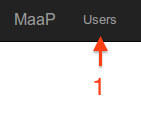
\includegraphics[width=0.2\textwidth]{img/usersButton.png}
					\caption{ \label{fig:pulsanteusers} Pulsante Users}
				\end{figure}

			% \item La index-page degli utenti (Figura \ref{fig:users}) visualizza gli utenti registrati nel sistema. 

			% 	\begin{figure}[H]
			% 		\centering 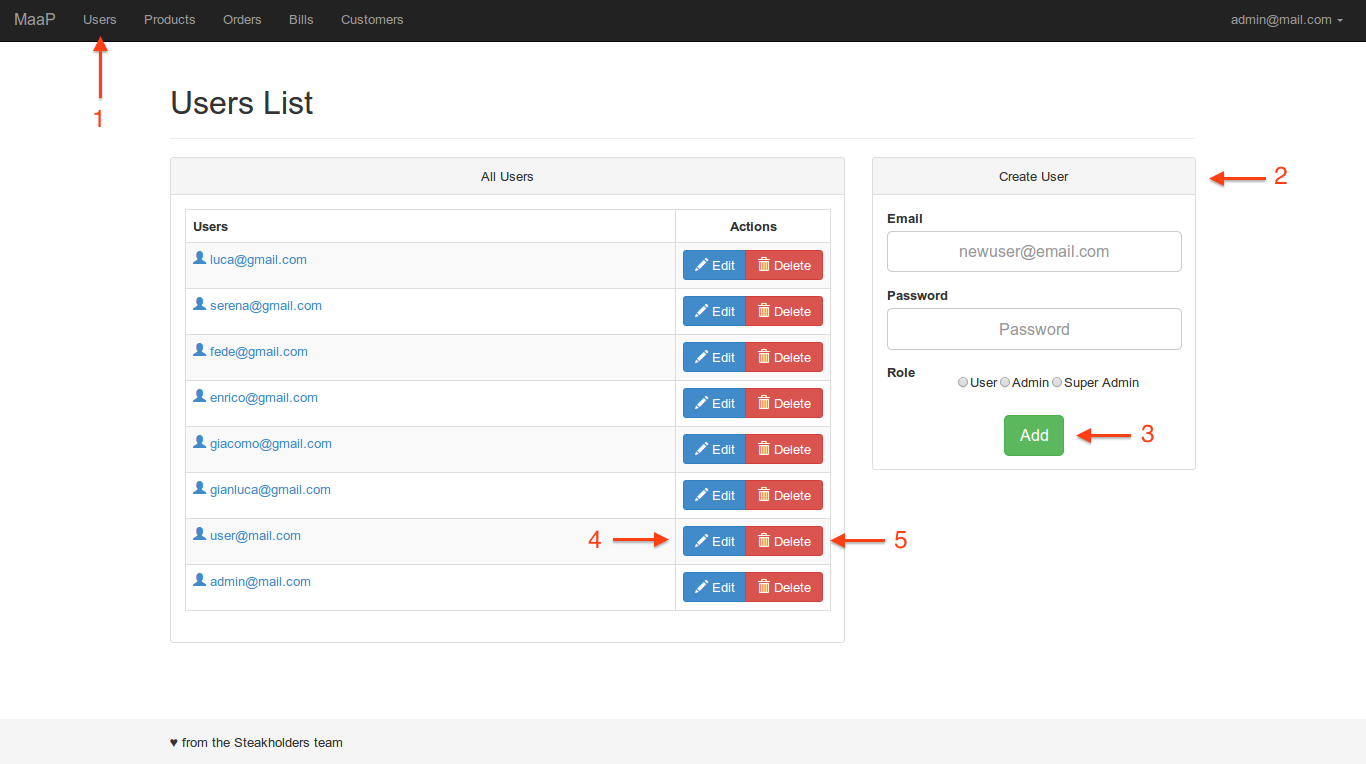
\includegraphics[width=0.8\textwidth]{img/users.png}
			% 		\caption{ \label{fig:users} Index-page degli utenti registrati}
			% 	\end{figure}

		% \end{enumerate}


	\clearpage
	\subsection{Visualizzazione show-page utente} % UCU 11.3
	\label{utenti-visualizzazione}
		\begin{enumerate}

			\item Per visualizzare la \glossario{show page} di un \glossario{utente} (Figura \ref{fig:usersEmailButton}) posizionarsi sulla \glossario{index-page} degli \glossario{utenti} come descritto in \ref{pulsanteusers}. Cliccare sull'attributo \emph{Users} (1) dell'utente di cui si vuole visualizzare la \glossario{show-page}.

				\begin{figure}[H]
					\centering 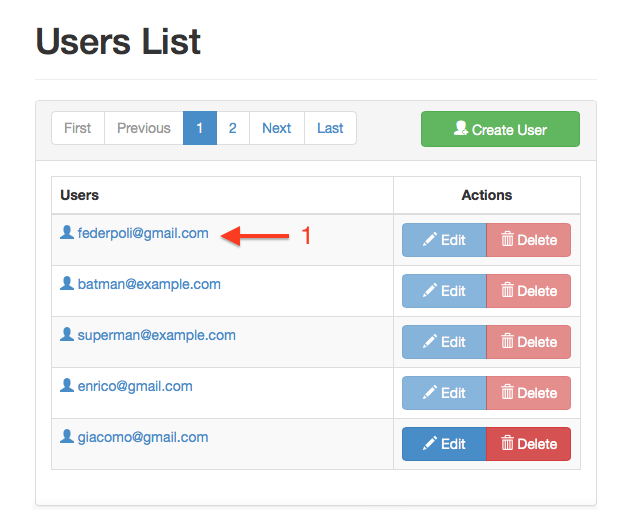
\includegraphics[width=0.8\textwidth]{img/usersEmailButton.png}
					\caption{ \label{fig:usersEmailButton} \glossario{Index-page} degli utenti registrati}
				\end{figure}

			\item Vengono visualizzati gli attributi dell'utente selezionato (Figura \ref{fig:userShowPage}).

				\begin{figure}[H]
					\centering 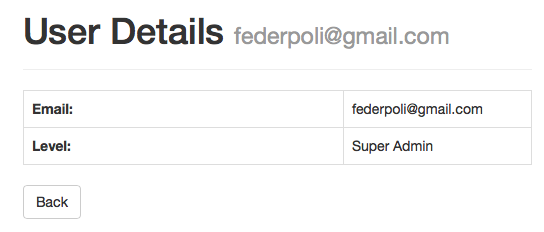
\includegraphics[width=0.8\textwidth]{img/userShowPage.png}
					\caption{ \label{fig:userShowPage} \glossario{Show-page} di un utente}
				\end{figure}

		\end{enumerate}

	\clearpage
	\subsection{Inserimento} % UCU 11.1
	\label{utenti-inserimento}
		\begin{enumerate}

			\item Per inserire un nuovo \glossario{utente} accedere alla index-page degli \glossario{utenti} (vedi \ref{visualizzaindexpageutenti}). Cliccare il pulsante \emph{Create User} (1) nella \glossario{collection-index} degli utenti (Figura \ref{fig:createuserButton}).
				\begin{figure}[H]
					\centering 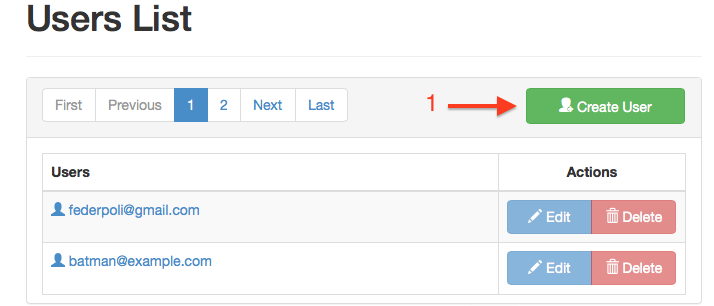
\includegraphics[width=0.8\textwidth]{img/createuserButton.png}
					\caption{ \label{fig:createuserButton} Pulsante di creazione utente}
				\end{figure}

			\item Inserire \emph{email} (1), \emph{password} (2), il livello \glossario{utente} (3) e confermare cliccando il pulsante \emph{Add User} (4). L'utente può annullare l'operazione cliccando sul pulsante \emph{Back} (5).

				\begin{figure}[H]
					\centering 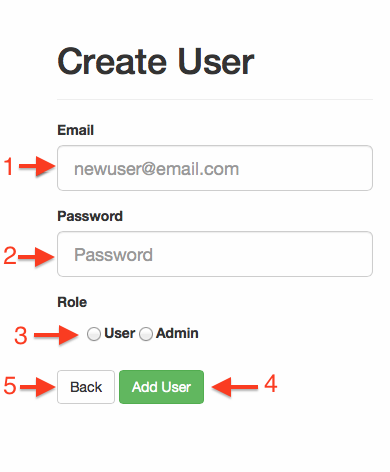
\includegraphics[width=0.5\textwidth]{img/formCreazioneUtente.png}
					\caption{ \label{fig:formCreazioneUtente} Form di creazione utente}
				\end{figure}

			\item Viene visualizzato un messaggio di conferma di avvenuta creazione \glossario{utente} (Figura \ref{fig:confermaCreazioneUtente}).

				\begin{figure}[H]
					\centering 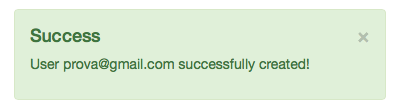
\includegraphics[width=0.5\textwidth]{img/confermaCreazioneUtente.png}
					\caption{ \label{fig:confermaCreazioneUtente} Messaggio conferma creazione \glossario{utente}}
				\end{figure}

		\end{enumerate}  

	\clearpage
	\subsection{Modifica} % UCU 11.3.1 e UCU 11.3.2
	\label{utenti-modifica}
		\begin{enumerate}

				\item Per modificare un \glossario{utente} accedere alla \glossario{index-page} degli utenti (vedi \ref{visualizzaindexpageutenti}). Cliccare il pulsante \emph{Edit} (1) nella \glossario{collection-index} degli utenti (Figura \ref{fig:editUserButton}).
					\begin{figure}[H]
						\centering 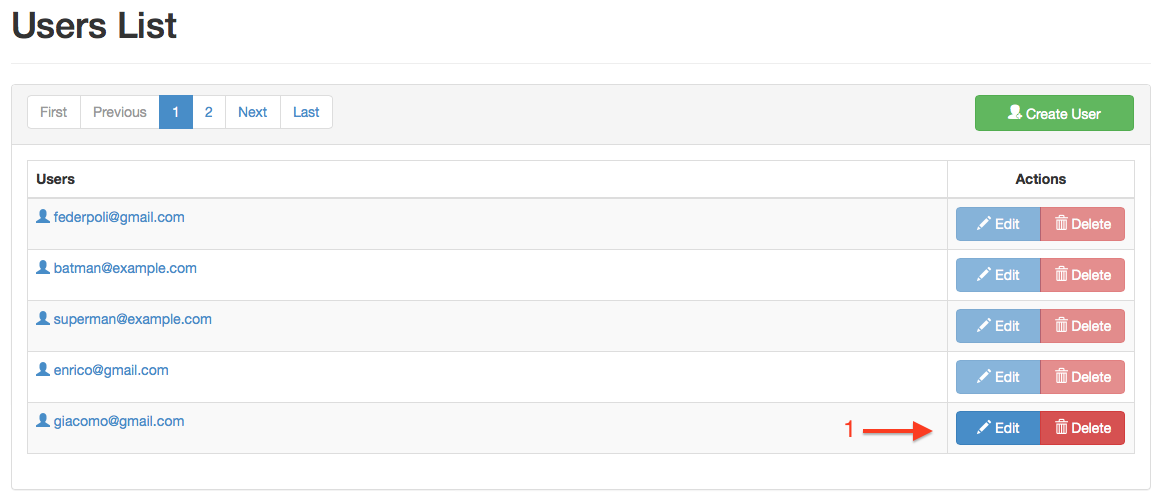
\includegraphics[width=0.8\textwidth]{img/editUserButton.png}
						\caption{ \label{fig:editUserButton} Pulsante di modifica \glossario{utente}}
					\end{figure}

				\item Viene proposto il form di modifica (Figura \ref{fig:editUserLevel}). Selezionare il livello \glossario{utente} desiderato tramite gli appositi selettori (1). L'utente può annullare l'operazione cliccando sul pulsante \emph{Cancel} (2).

					\begin{figure}[H]
						\centering 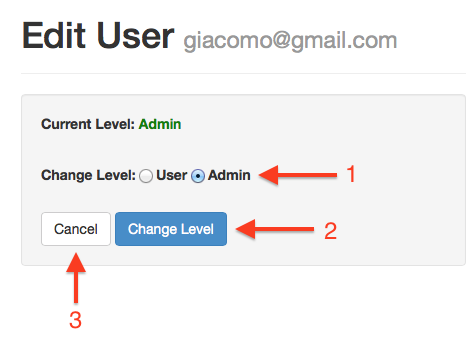
\includegraphics[width=0.6\textwidth]{img/editUserLevel.png}
						\caption{ \label{fig:editUserLevel} Form di modifica utente}
					\end{figure}

				\item Viene visualizzato un messaggio di conferma di avvenuta modifica utente (Figura \ref{fig:confirmEditUser}).

					\begin{figure}[H]
						\centering 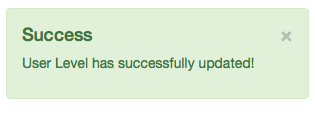
\includegraphics[width=0.5\textwidth]{img/confirmEditUser.png}
						\caption{ \label{fig:confirmEditUser} Messaggio conferma modifica utente}
					\end{figure}

			\end{enumerate}  
	
	\clearpage
	\subsection{Eliminazione} % UCU 11.3.3
	\label{utenti-eliminazione}
		\begin{enumerate}

				\item Per eliminare un \glossario{utente} accedere alla \glossario{index-page} degli utenti (vedi \ref{visualizzaindexpageutenti}). Cliccare il pulsante \emph{Delete} (1) nella \glossario{collection-index} degli utenti (Figura \ref{fig:deleteUserButton}).
					\begin{figure}[H]
						\centering 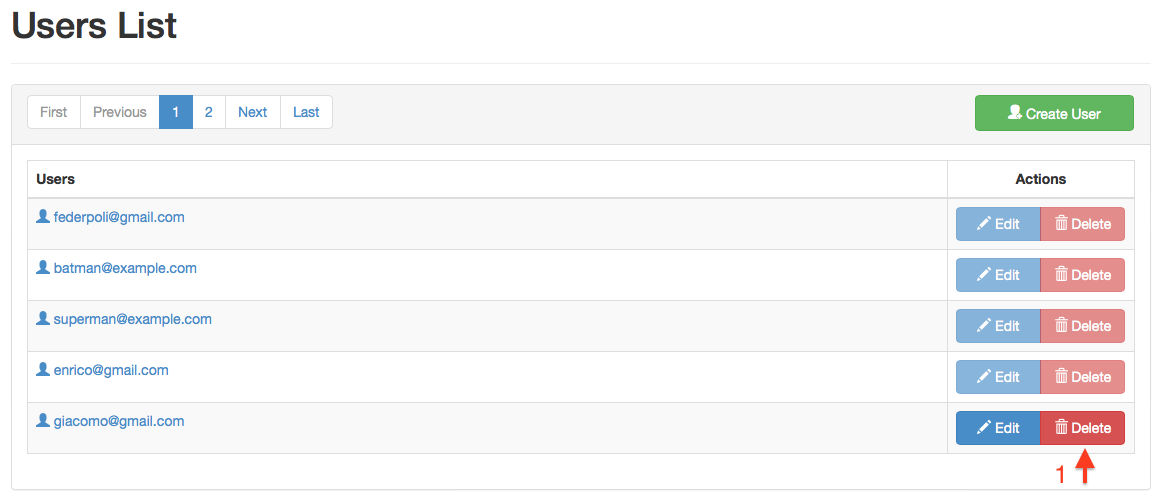
\includegraphics[width=1\textwidth]{img/deleteUserButton.png}
						\caption{ \label{fig:deleteUserButton} Pulsante elimina utente}
					\end{figure}

				\item Viene chiesta conferma (Figura \ref{fig:confirmDeleteUser}) prima di procedere con la cancellazione dell \glossario{utente} selezionato.

					\begin{figure}[H]
						\centering 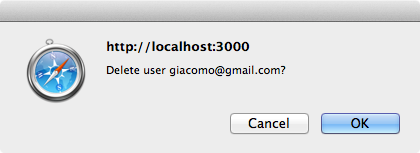
\includegraphics[width=0.6\textwidth]{img/confirmDeleteUser.png}
						\caption{ \label{fig:confirmDeleteUser} Form di modifica utente}
					\end{figure}

				\item Viene visualizzato un messaggio di conferma di avvenuta eliminazione utente (Figura \ref{fig:messageDeletedUser}).

					\begin{figure}[H]
						\centering 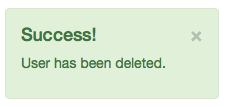
\includegraphics[width=0.5\textwidth]{img/messageDeletedUser.png}
						\caption{ \label{fig:messageDeletedUser} Messaggio conferma eliminazione utente}
					\end{figure}

			\end{enumerate}  
		